\chapter{Psykoakustik}

Frekvensspektret for menneskets hørelse omtales ofte som værende fra ca. 20Hz - 20kHz. \cite{Elektroakustik}. Dog opfatter øret ikke alle frekvenser lige godt, da vores hørelse ikke blot er afhængig af frekvensen, men også af lydtrykket. Specielt for lave frekvenser skal lydtrykket øges betragteligt for at lydopfattelsen er den samme, som ved mellem- eller højefrekvenser. Lydtrykket måles i dB, med den menneskelige høretærskel ($20\mu Pa$)  som reference, og omtales ofte som SPL dB (Sound pressure level). Figur \ref{fig:SPL} viser netop, at en tone på f.eks 1000Hz kræver et lydtryk på 30 SPL dB for en relativ lydopfattelse på 30phon, mens der for en tone på 63Hz kræves et lydtryk på ca 65 SPL dB for samme opfattelse af lydniveauet på 30phon.

\begin{figure}[h!]
	\centering
	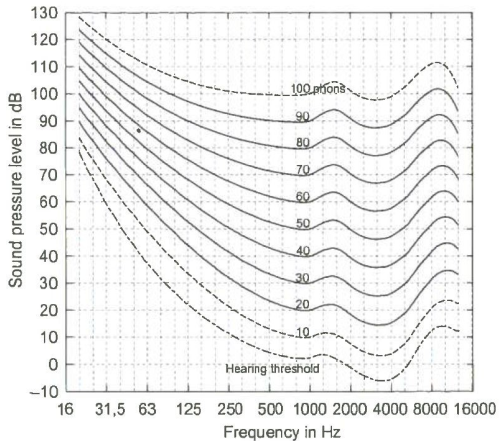
\includegraphics[width=.6\textwidth]{Pics/SPL.PNG}
	\label{fig:SPL}
	\caption{Det menneskelige øres opfattelse af lyd. \cite{Elektroakustik}}
\end{figure}

I en normal dagligdag, er dette ikke det store problem, da de lyde vi primært skal forholde os til (tale, dyrelyde, trafik- og omgivelsesstøj) ligger i mellemtone spektret (ca. \SI{500}{\hertz} - \SI{6000}{\hertz}). 

Mange mennesker ynder dog at lytte til musik, hvor det her er muligt at frembringe toner helt ned til under \SI{30}{\hertz}. For at få den fulde oplevelse af lyden i både bund og top af frekvensspektret, arbejdes der ihærdigt på at øge SPL af de lave frekvenser uden at mellem- og højtonerne ryger op i et lydtryk på 140 SPL dB, som er smertegrænsen for det menneskelige øre.